\documentclass[11pt,letterpaper]{article}
\usepackage[lmargin=1in,rmargin=1in,bmargin=1in,tmargin=1in]{geometry}
\usepackage{style/quiz}
\usepackage{style/commands}

% -------------------
% Content
% -------------------
\begin{document}
\thispagestyle{title}


% Quiz 1
\quizsol \textit{True/False}: The following relation represents a function:
	\[
	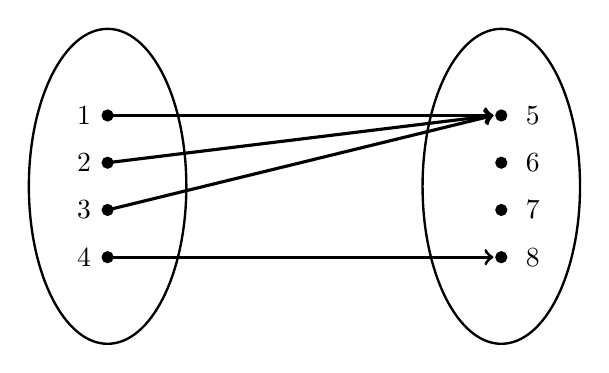
\begin{tikzpicture}
	% Ellipses
	\draw[line width=0.03cm] (0,0) circle (1 and 2);
	\draw[line width=0.03cm] (5,0) circle (1 and 2);
	
	% Nodes
	\draw[fill=black] (0,0.9) circle (0.07);
	\draw[fill=black] (0,0.3) circle (0.07);
	\draw[fill=black] (0,-0.3) circle (0.07);
	\draw[fill=black] (0,-0.9) circle (0.07);
	
	\draw[fill=black] (5,0.9) circle (0.07);
	\draw[fill=black] (5,0.3) circle (0.07);
	\draw[fill=black] (5,-0.3) circle (0.07);
	\draw[fill=black] (5,-0.9) circle (0.07);
	
	% Arrow
	\draw[line width=0.04cm,->] (0,0.9) -- (4.9,0.9);
	\draw[line width=0.04cm,->] (0,0.3) -- (4.9,0.9);
	\draw[line width=0.04cm,->] (0,-0.3) -- (4.9,0.9);
	\draw[line width=0.04cm,->] (0,-0.9) -- (4.9,-0.9);
	
	% Labels
	\node at (-0.3,0.9) {$1$};
	\node at (-0.3,0.3) {$2$};
	\node at (-0.3,-0.3) {$3$};
	\node at (-0.3,-0.9) {$4$};
	
	\node at (5.4,0.9) {$5$};
	\node at (5.4,0.3) {$6$};
	\node at (5.4,-0.3) {$7$};
	\node at (5.4,-0.9) {$8$};
	\end{tikzpicture}
	\]

\sol The statement is \textit{true}. A relation is a function if for every input, i.e. every value in the domain, there is one output. For each of the values 1, 2, 3, 4, we know the value of the output. It does not matter that several of the values get `sent' to the same value---only that we know what value they go to. \pvspace{1.5cm}



% Quiz 2
\quizsol \textit{True/False}: If $C(x)$ is a cost function, then the $y$-intercept of $C(x)$ is the fixed costs. \pspace

\sol The statement is \textit{true}. The $y$-intercept of a function is the value where $x= 0$ (which means the function is intersecting the $y$-axis). But then we are looking at the value of $C(0)$, which represents the costs of producing zero items. But any costs associated with producing zero items must be a `baseline' cost for production, i.e. the fixed costs. \pvspace{1.5cm}



% Quiz 3
\quizsol \textit{True/False}: The point $(1, 1)$ is the solution to the system of equations:
	\[
	\begin{aligned}
	2x + y&= 3 \\
	x - y&= 1
	\end{aligned}
	\]

\sol The statement is \textit{false}. The simplest way of seeing this is to check if $(x,y)= (1,1)$ is a solution to the system, i.e. check if $x= 1$ and $y= 1$ satisfies both equations: $2(1) + 1= 3$ but $1 - 1= 0 \neq 1$. Therefore, $(1, 1)$ is not the solution to the system of equations. We can also determine if $(1, 1)$ is a solution to the system of equations by solving the system: \par
	\begin{table}[!ht]
	\centering
	\begin{tabular}{cccc}
	& $2x + y$ & $=$ & $3$ \\
	& $x - y$ & $=$ & $1$ \\ \hline
	& $3x$ & $=$ & $4$ \\
	& $x$ & $=$ & $4/3$ 
	\end{tabular}
	\end{table}
Then certainly, we cannot have $x= 1$. We then can find that $y= x - 1= 4/3 - 1= 1/3$. Then the correct solution is $(x, y)= (4/3, 1/3)$. 



\newpage



% Quiz 4
\quizsol \textit{True/False}: If $P(x)$ is a profit function, then $P(0)$ is a breakeven point. \pspace

\sol The statement is \textit{false}. Recall that a breakeven point is when revenue, $R(x)$, equals cost, $C(x)$. But this is $R(x)= C(x)$. This is the same as $R(x) - C(x)= 0$. But $P(x)= R(x) - C(x)$ so that $P(x)= 0$. Alternatively, a breakeven point can be defined as a $x$ value when the profit is 0, i.e. $P(x)= 0$. \pvspace{1.5cm}



% Quiz 5
\quizsol \textit{True/False}: Consider the following system of equations:
	\[
	\begin{aligned}
	2x + 3y&= -1 \\
	x - 2y&= 5
	\end{aligned}
	\]
Then the associated augmented matrix is 
	\[
	\begin{pmatrix}
	2 & 3 & -1 \\
	1 & -2 & 5
	\end{pmatrix}
	\]

\sol The statement is \textit{true}. Remember, the augmented matrix is the matrix consisting of all the coefficients for the variables (`in order') in each equation for each of the equations (`in order'). Then the to right of the rightmost column, we add (augment) the matrix with the solution vector, i.e. the vector of the solutions for the equations (`in order'). Applying this to the given system of equations, we obtain exactly
	\[
	\begin{pmatrix}
	2 & 3 & -1 \\
	1 & -2 & 5
	\end{pmatrix}
	\] \pvspace{1.5cm}



% Quiz 6
\quizsol \textit{True/False}: A system of solutions to the system of equations given by the augmented matrix
	\[
	\begin{pmatrix}
	1 & 0 & 0 & 1 & 2 \\
	0 & 1 & 0 & -3 & -1 \\
	0 & 0 & 1 & 0 & 0 
	\end{pmatrix}
	\]
is $x_3= 0$, $x_4= \text{free}$, $x_1= 2 - x_4$, and $x_2= 3x_4 - 1$. \pspace

\sol The statement is \textit{true.} First, observe that the matrix is in reduced row echelon form so that we should be read iff the solutions. Because the matrix is augmented, each column (except the last) of the matrix corresponds to one of the variables and the last column corresponds to the solution to each of the corresponding equation. Writing out the corresponding system of equations, we have
	\[
	\begin{aligned}
	1x_1 + 0x_2 + 0x_3 + 1x_4&= 2 \\
	0x_1 + 1x_2 + 0x_3 - 3x_4&= -1 \\
	0x_1 + 0x_2 + 1x_3 + 0x_4&= 0
	\end{aligned}
	\]
which of course is equivalent to\dots
	\[
	\begin{aligned}
	x_1 + x_4&= 2 \\
	x_2 - 3x_4&= -1 \\
	x_3&= 0
	\end{aligned}
	\]
From this system, we see that $x_3= 0$. Letting $x_4$ be free, we see that $x_1= 2 - x_4$ and $x_2= 3x_4 - 1$. But then a system of solutions to the equations is
	\[
	\begin{aligned}
	x_1&= 2 - x_4 \\
	x_2&= 3x_4 - 1 \\
	x_3&= 0 \\
	x_4&: \text{free}
	\end{aligned}
	\] \pvspace{1.5cm}



% Quiz 7
\quizsol \textit{True/False}: If $A$ is a $5 \times 3$ matrix and $B$ is a $3 \times 6$ matrix, you can compute $AB$, which will be a $3 \times 6$ matrix. \pspace

\sol The statement is \textit{false}. Recall that a $n \times m$ matrix $A$ and a $p \times q$ matrix $B$ can be multiplied if $m= p$. If so, they form a $n \times q$ matrix. So while we can multiply $A$ and $B$, they form a $5 \times 6$ matrix. 
	\[
	\begin{tikzpicture}
	\node at (1.3,2.2) {If $\to$ matches $\downarrow$};
	\node at (1.3,-2.2) {Produces $\leftarrow$ and $\uparrow$ matrix.};
	
	\draw[->,line width=0.03cm] (-0.75,1.5) -- (0.50,1.5);
	\draw[->,line width=0.03cm] (3.5,0.5) -- (3.5,-0.5);
	
	\draw[->,line width=0.03cm] (3,-1.5) -- (1,-1.5);
	\draw[->,line width=0.03cm] (-1,-1) -- (-1,1);
	
	\node at (0,0) {$\begin{pmatrix} &&\\&&\\&&\\&&\\&& \end{pmatrix}$};
	\node at (2,0) {$\begin{pmatrix} &&&&& \\ &&&&& \\ &&&&& \end{pmatrix}$};
	\end{tikzpicture}
	\] \pvspace{1.5cm}



% Quiz 8
\quizsol \textit{True/False}: If $\det A= 0$, then $A$ does not have an inverse. \pspace

\sol The statement is \textit{true}. If $\det A= 0$, then $A$ does not have an inverse. Conversely, it is true that if $A$ does not have an inverse that $\det A= 0$. Therefore, if $A$ has an inverse, then $\det A \neq 0$ and that if $\det A \neq 0$, then $A$ has an inverse. \pspace



% Quiz 9 
\quizsol \textit{True/False}: For any matrix $A$, if we have $Ax= b$, then $x= A^{-1}b$. \pspace

\sol The statement is \textit{false}. For $A^{-1}$ to exist, the matrix $A$ needs to be invertible. If $A$ is invertible, then $A^{-1}$ exists. But then we have
	\[
	\begin{aligned}
	Ax&= b \\
	A^{-1}Ax&= A^{-1}b \\
	I_nx&= A^{-1}b \\
	x&= A^{-1}b
	\end{aligned}
	\]
Not all matrices are invertible. 



\newpage



% Quiz 10
\quizsol \textit{True/False}: Any function on a nonempty region given by a collection of inequalities has a maximum and minimum value which occur at a corner point of the region. \pspace

\sol The statement is \textit{true}. This is the Fundamental Theorem of Linear Programming. \pvspace{1.5cm}



% Quiz 11
\quizsol \textit{True/False}: The pivot position is given by the entry whose column contains the most negative entry in the bottom row and the smallest positive ratio in its row. \pspace

\sol The statement is \textit{true}. This is the procedure to choose the pivot position. For instance, in the tableau below, the most negative entry in the bottom row is in the third column. Using the third column and examining the ratios in each rows, we see that the second row has the smallest \textit{positive} ration. 
	\begin{table}[!ht]
	\centering
	\begin{tabular}{rrrrr|rr}
	$5$ & $-2$ & $3$ & $1$ & $-4$ & $9$ & \quad {\footnotesize $9/3= 3$} \\
	$-1$ & $0$ & \textcircled{$5$} & $6$ & $2$ & $10$ & \quad {\footnotesize $10/5= 2$} \\
	$6$ & $1$ & $2$ & $0$ & $-5$ & $-20$ & \quad {\footnotesize $-20/2= -10$} \\ \cline{1-6}
	$8$ & $0$ & $-4$ & $1$ & $-3$ & $0$ & \\
	\end{tabular}
	\end{table} \par
Therefore, the circled entry is the pivot position. \pvspace{1.5cm}



% Quiz 12
\quizsol \textit{True/False}: Every linear programming minimization problem in standard form has a dual maximization problem. \pspace

\sol The statement is \textit{true}. This is sometimes known as the Fundamental Theorem of Duality. \pvspace{1.5cm}












\end{document}